\chapter{Classification Method}
\label{ch:method}

\section{Nonparametric Supervised Learning}

% TODO: Add some perspective

Suppose we have a space of objects $\Omega$, a set of class labels $Z$, and a
probability distribution $\mu$ on $\Omega \times Z$. For simplicity, we take the
classes to be $+$ and $-$. Based on objects $X$ and labels $Y$ drawn from $\mu$,
we would like to learn a classification function that maps each object to its
correct class label. This is the standard supervised learning problem.

Typically, when one wants to learn a model of how objects map to labels one
selects some model space and chooses the the best model from that model space,
prefering a model that fits the data but is not too complex. The choice of model
space encodes assumptions about the problem. For example, in the class of
methods known as Tikhonov Regularization \cite{Poggio}, of which Support Vector
Machines and Regularized Least Squares are special cases, this choice manifests
itself in the choice of a kernel and its associated Reproducing Kernel Hilbert
Space. 

There are many ways to specify a model and therefore many types of model
spaces. Tikhonov Regularization specifies the model as a function. It defines
model complexity using the norm of the function in RKHS. Then it searches over
the RKHS to find the best function. However, the model need not be specified by
a function in a function space at all. It could be specified by a neural network
with a certain architecture, or a spline with a certain number of nodes, or a
boolean expression with a certain number of terms. Each of these settings have
corresponding ways to determine model complexity and to do model selection.

With this in mind, we propose a setting for model specification and selection in
supervised learning based on a {\em latent source model}. In this setting, the
model is specified by a small collection of unknown {\em latent sources}. We
posit that the data were generated by the latent sources according to a
stochastic model relating latent sources and observations.

% The choice of model induces some structure in the classification
      % function. However, we are entirely unaware of the structure...etc

Rather than encoding any assumptions about the data via a choice of model space
(e.g. all sets of 10 latent sources) and searching over the model space for the
best set of latent sources, we rely directly on the data itself as a proxy for
the unknwon latent sources.

However, rather than searching over the entire model space, we propose a
classification method that functions without any prior knowledge of what the
latent sources are or how many there are. Instead, our method relies on large
amounts of data as a proxy for the unknown latent sources. We perform
classification by directly computing the conditional class probabilities for an
observation based on our stochastic model. This approach results in a surprising
and natural interpretation --- that to see how likely it is that an observation
belongs to a certain class, we can simply observe how much it resembles other
examples of that class. This is well-suited to problems with large amounts of
labeled data.


Suppose, however, that we are entirely unaware of the structure of the
classification function. To resolve this, we propose the following nonparametric
model relating observed objects to their labels. We posit that there are a
relatively small number of distinct {\em latent source} objects in each class
that account for all observed objects in that class. Let us call them $\mb t_1,
\dots, \mb t_n$ for $+$ and $\mb q_1, \dots, \mb q_{\ell}$ for $-$. Each
observation labeled $+$ is assumed to be a noisy version of one of the latent
sources $\mb t_1, \dots, \mb t_n$. Similarly, each observation labeled $-$ is
assumed to be a noisy version of one of the latent sources $\mb q_1, \dots \mb
q_{\ell}$. We do not know what the latent objects are or even how many there
are. We only know the stochastic model that relates an observation to its latent
source object.

\section{Stochastic Model}
To make the presentation more concrete, let us focus for the rest of this
chapter on time-varying {\em signals} --- the main objects of concern in this
thesis. In this context, an observed object is simply a signal in a time window
of a certain length.  A latent source object may be thought of as a signal
corresponding to a prototypical type of event. If the same type of event were to
happen many times, we suppose that the resulting observed signals are noisy
versions of the latent source signal corresponding to that type of event.

We say an observation $\mb s$ is {\em generated} by a latent source $\mb q$ if $\mb s$
is a noisy version of $\mb q$. Accordingly, we propose the following stochastic
model relating a latent source $\mb q$ and an observation $\mb s$:
\begin{gather}
\pr(\mb s \text{ generated by } \mb q) = \exp\left(-\gamma d(\mb s,\mb q) \right)
\end{gather}
where $d(\mb s, \mb q)$ is the {\em distance} between $\mb s$ and $\mb q$ and $\gamma$ is a
scaling parameter. This coincides with the notion that the closer an observation
is to a latent source, the more likely it is that the observation came from that
source. For example, a choice of distance function might be
\begin{gather}
d(\mb s,\mb q) = \sum_{i=1}^{N_{obs}} (s_i - q_i)^2
\end{gather}
for digital signals $\mb s$ and $\mb q$ of length $N_{obs}$. However, any
symmetric, positive definite, and convex $d$ would work.
%TODO: you also assume later that it's a norm.

\section{Detection}
\subsection{Class Probabilities}
Suppose that $\mb s$ is an observed signal of length $N_{obs}$. We would like to
compute the probability that $\mb s$ belongs to each class. We can then use
those probabilities to compute an estimate of the class of $\mb s$.  To compute
the probability that $\mb s$ belongs to each class, we make use of a set of {\em
  reference} signals for each class --- a set $\mathcal{R}_+$ of signals sampled
from $+$ and a set $\mathcal{R}_-$ of signals sampled from $-$. Reference
signals represent historical data about previous activity from each class to
which we can compare our observation and draw conclusions about which class it
belongs to. We will assume that reference signals have length $N_{ref} \geq
N_{obs}$. We will deal with the case of $N_{ref} = N_{obs}$ first and generalize
in the following section.

Under our model the observation must belong to $+$ if it has the same
latent source as one of the reference signals in $\mathcal{R}_+$. Similarly, the
observation must belong to $-$ if it has the same latent source as one of the
reference signals in $\mathcal{R}_-$. Hence, the probability that the
observation belongs to $+$ is
\begin{align}
\pr(+ \;|\; \mb s) &= \sum_{\mb r \in \mathcal{R}_+} \pr(\mb s \text{ belongs to } +, \mb s \text{ shares a latent source
  with } \mb r)\notag\\
&= \sum_{\mb r \in \mathcal{R}_+} \sum_{j = 1}^n \pr( \mb s \text{ generated by }
\mb t_j, \mb r \text{ generated by } \mb t_j)\notag\\
&= \sum_{\mb r \in \mathcal{R}_+} \sum_{j = 1}^n \exp{\left(-\gamma
    d(\mb s,\mb t_j)\right)} \exp{\left(-\gamma d(\mb r,\mb t_j)\right)}\notag\\
&= \sum_{\mb r \in \mathcal{R}_+} \sum_{j = 1}^n \exp{\left(-\gamma\left(
    d(\mb s,\mb t_j) + d(\mb r,\mb t_j) \right)\right)}
\end{align}
For large enough $\gamma$, the term with the smallest exponent will dominate the sum
over the latent sources and we can write
\begin{align}
\pr(+ \;|\; \mb s) &\approx \sum_{\mb r \in \mathcal{R}_+}
\exp{\left(-\gamma \min_{j} \left( d(\mb s,\mb t_j) + d(\mb r,\mb t_j) \right) \right)} \label{eqn:prob_plus}
\end{align}
However, the expression so far still involves a minimization over the unknown
latent sources $\mb t_j$. We would like to eliminate the $\mb t_j$ altogether
and just end up with a sum over all reference signals $\mb r$. If we suppose
that the space of signals is reasonably well-covered by the latent sources, then
the minimizing source $\mb t_{j^*}$ should be close to the global minimizer
$\mb t^*$ over all signals. Figure \ref{fig:conv_comb} illustrates the reference
signal $\mb r$, the observation $\mb s$, the latent source signals $\mb t_1, \dots,
\mb t_n$, and the minimizing latent source signal $\mb t_{j^*}$.
\begin{figure}[h!]
\begin{center}
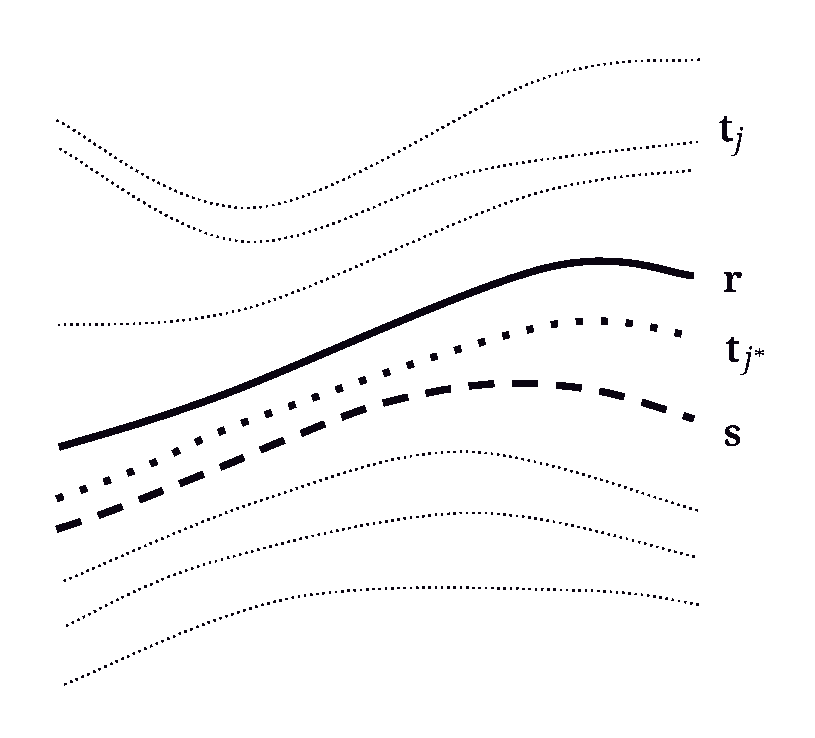
\includegraphics[width=3in]{latentsources}
\end{center}
\caption{\label{fig:conv_comb} An illustration of the latent source signal
  $\mb t_{j^*}$ that minimizes $d(\mb s,\mb t_j) + d(\mb r,\mb t_j)$ in
  Eq. \ref{eqn:prob_plus}. Depicted are the reference signal $\mb r$, the
  observation $\mb s$, the latent source signals $\mb t_1, \dots, \mb t_n$, and the
  minimizing latent source signal $\mb t_{j^*}$.}
\end{figure}

The global minimizer $\mb t^*$ is simply the mean of $\mb s$ and $\mb t$. To see
this, first observe that since $d(\mb s,\mb t)$ and $d(\mb r, \mb t)$ are convex
in $\mb t$, $d(\mb s,\mb t) + d(\mb r,\mb t)$ is also convex in $\mb t$. Second,
let us assume that the distance function $d(\mb s,\mb t)$ is actually a {\em
  norm} and therefore has the functional form $d(\mb s,\mb t) = c(\mb s-\mb t)$,
which depends only on the difference between signals. Finally, observe that
\begin{align}
\frac{\partial}{\partial \mb t} \left(d(\mb s,\mb t) + d(\mb r,\mb t)\right)\Big|_{\mb t = \frac{\mb s + \mb r}{2}}
&= \frac{\partial}{\partial \mb t}\left(c\left(\mb t - \mb s\right) + c\left(\mb t-\mb r\right)\right)\Big|_{\mb t = \frac{\mb s + \mb r}{2}}\notag\\
&= c'\left(\frac{\mb s+\mb r}{2} - \mb s\right) + c'\left(\frac{\mb s+\mb r}{2}-\mb r\right)\notag\\
&= c'\left(\frac{\mb r-\mb s}{2}\right) + c'\left(\frac{\mb s-\mb r}{2}\right)\notag\\
&= 0
\end{align}
where in the last line, we have made use of the symmetry of $c$ induced by the symmetry of $d$.

Because $d(\mb s, \mb t) + d(\mb r, \mb t)$ is convex in $\mb t$ and the
derivative with respect to $\mb t$ at $\frac{\mb s + \mb r}{2}$ is zero, $\mb
t^* = \frac{\mb s + \mb r}{2}$ is indeed the global minimizer. Now, we can
compute the corresponding global minimum $d(\mb s,\mb t^*) + d(\mb r,\mb
t^*)$. The global minimum is
\begin{align}
d(\mb s,\mb t^*) + d(\mb r,\mb t^*) &= d\left(\mb s,\frac{\mb r + \mb s}{2}\right) + d\left(\mb r,\frac{\mb r + \mb s}{2}\right)\notag\\
&= c\left(\frac{\mb r - \mb s}{2}\right) + c\left(\frac{\mb s - \mb r}{2}\right) \label{eqn:th_min1}
\end{align}
Let us also assume that for any reasonable distance function $c$, scaling the
argument by a constant scales the distance according to
\begin{gather}
c(a\mb x) = g(a)c(\mb x)
\end{gather}
where $g$ is some positive definite function. Applying this to Eq. \ref{eqn:th_min1} gives
\begin{align}
d(\mb s,\mb t^*) + d(\mb r,\mb t^*) &= g\left(\frac{1}{2}\right) c(\mb r - \mb s) +  g\left(\frac{1}{2}\right) c(\mb s - \mb r)\notag\\
&= 2 \cdot g\left(\frac{1}{2}\right) c(\mb r - \mb s)\notag\\
&= 2 \cdot g\left(\frac{1}{2}\right) d(\mb r, \mb s)\notag\\
&= C \cdot d(\mb r, \mb s).
\end{align}
where $C$ is a constant independent of $\mb r$ and $\mb s$.

Having done this, we can now approximate $\min_j (d(\mb s,\mb t_j) + d(\mb r,\mb
t_j))$ in Eq. \ref{eqn:prob_plus} by $C \cdot d(\mb s,\mb r)$, assuming the
actual minimizing latent source $t_{j^*}$ is close to the global minimizer
$\mb t^*$. This gives us the probability that the observation belongs to $+$ without
having to minimize over the unknown $\mb t_j$:
\begin{align}
\pr(+ \;|\;\mb s) &\approx \sum_{\mb r \in \mathcal{R}_+}
\exp{\left(-\gamma \min_{j} \left( d(\mb s,\mb t_j) + d(\mb r,\mb t_j) \right) \right)}\notag\\
&\approx \sum_{\mb r \in \mathcal{R}_+} \exp
\left(-\gamma d(\mb s,\mb r)\right) \label{eqn:prob_plus_approx}
\end{align}
where we have absorbed $C$ into $\gamma$ for convenience. We can similarly compute the probablity that the observation belongs to $-$:
\begin{align}
\pr(- \;|\; \mb s ) &\approx \sum_{\mb r \in
  \mathcal{R}_-} \exp \left(-\gamma d(\mb s,\mb
  r)\right) \label{eqn:prob_minus_approx}
\end{align}

\subsection{Class Estimator}
Our class estimation rule is simple: assign to the obsevation the class with the
highest probability. In practice, we compute the ratio of $\pr(+ \;|\; \mb s)$
and $\pr(- \;|\; \mb s)$ 
\begin{gather}
R(\mb s) = \frac{\pr(+ \;|\; \mb s)}{\pr(- \;|\; \mb s)} = \frac{\displaystyle \sum_{\mb r \in \mathcal{R}_+} \exp \left(-\gamma d(\mb s,\mb r)\right)}{\displaystyle \sum_{\mb r \in \mathcal{R}_-} \exp \left(-\gamma d(\mb s,\mb r)\right)}
\end{gather}
and check if it exceeds a threshold of $\theta = 1$. For a quadratic distance function, this becomes
\begin{gather}
R(\mb s) = \frac{\displaystyle \sum_{\mb r \in \mathcal{R}_+} \exp \left(-\gamma \displaystyle \sum_{i=1}^{N_{obs}} (s_i - r_i)^2\right)}{\displaystyle \sum_{\mb r \in \mathcal{R}_-} \exp \left(-\gamma \displaystyle \sum_{i=1}^{N_{obs}} (s_i - r_i)^2\right)}
\end{gather}
The estimator for the class label $L$ is therefore
\begin{gather}
\hat{L}(\mb s) = \left\{
\begin{array}{ll}
+ & \text{if } R(\mb s) > \theta\\
- & \text{if } R(\mb s) \leq \theta.
\end{array}
\right.
\end{gather}
In practice, values other than 1 may also be used for the threshold $\theta$. For
example, if the benefits of true positives outweigh the costs of false
positives, one may set $\theta$ to less than 1. On the other hand, if the
costs of false positives outweigh the benefits of true positives, one may
conservatively set $\theta$ to greater than 1. We explore this effect in
Chapter \ref{ch:results}.

\subsubsection{Accumulating Evidence}
In some cases, for example when dealing with noisy data, it could be
advantageous to accumulate evidence over multiple timesteps before determining
which class the observation belongs to. A simple extension of our algorithm
would be to require that the observation is judged to belong to a particular
class for several consecutive timesteps. We shall call this number of required
timesteps $D_{req}$. We study the effect of $D_{req}$ in Chapter \ref{ch:results.}

\subsection{Online Classification}
In the previous sections, we have assumed that the reference signals and the
observations have the same length. In the online classification setting, it is
convenient to extend this to reference signals of arbitrary length. At its core,
our method compares an observation --- recently observed measurements of some
property of a system --- to reference signals --- sets of historical
measurements of that property for each class. Recently observed measurements are
judged to belong to the class whose reference signals they most resemble. For
reference signals and observations of the same size, this resemblence is
computed using the distance function $d$ previously described. In practice,
however, there are two complications. The first complication is that
observations will generally be short, containing a small amount of recent
samples, and reference signals will be long, containing large amounts of
historical data. The second complication is that reference signals will often
have unknown phase. That is, the events underlying the reference signals may
have occurred at arbitrary time shifts with respect to one another. Furthermore,
when comparing the observation to each reference signal, there is no temporal
point of reference between the two. A natural solution to both of these
complications is to check whether the observation resembles any {\em piece} of
the reference signal of the same size as the observation. Figure
\ref{fig:mindist} illustrates this.
\begin{figure}
\begin{center}
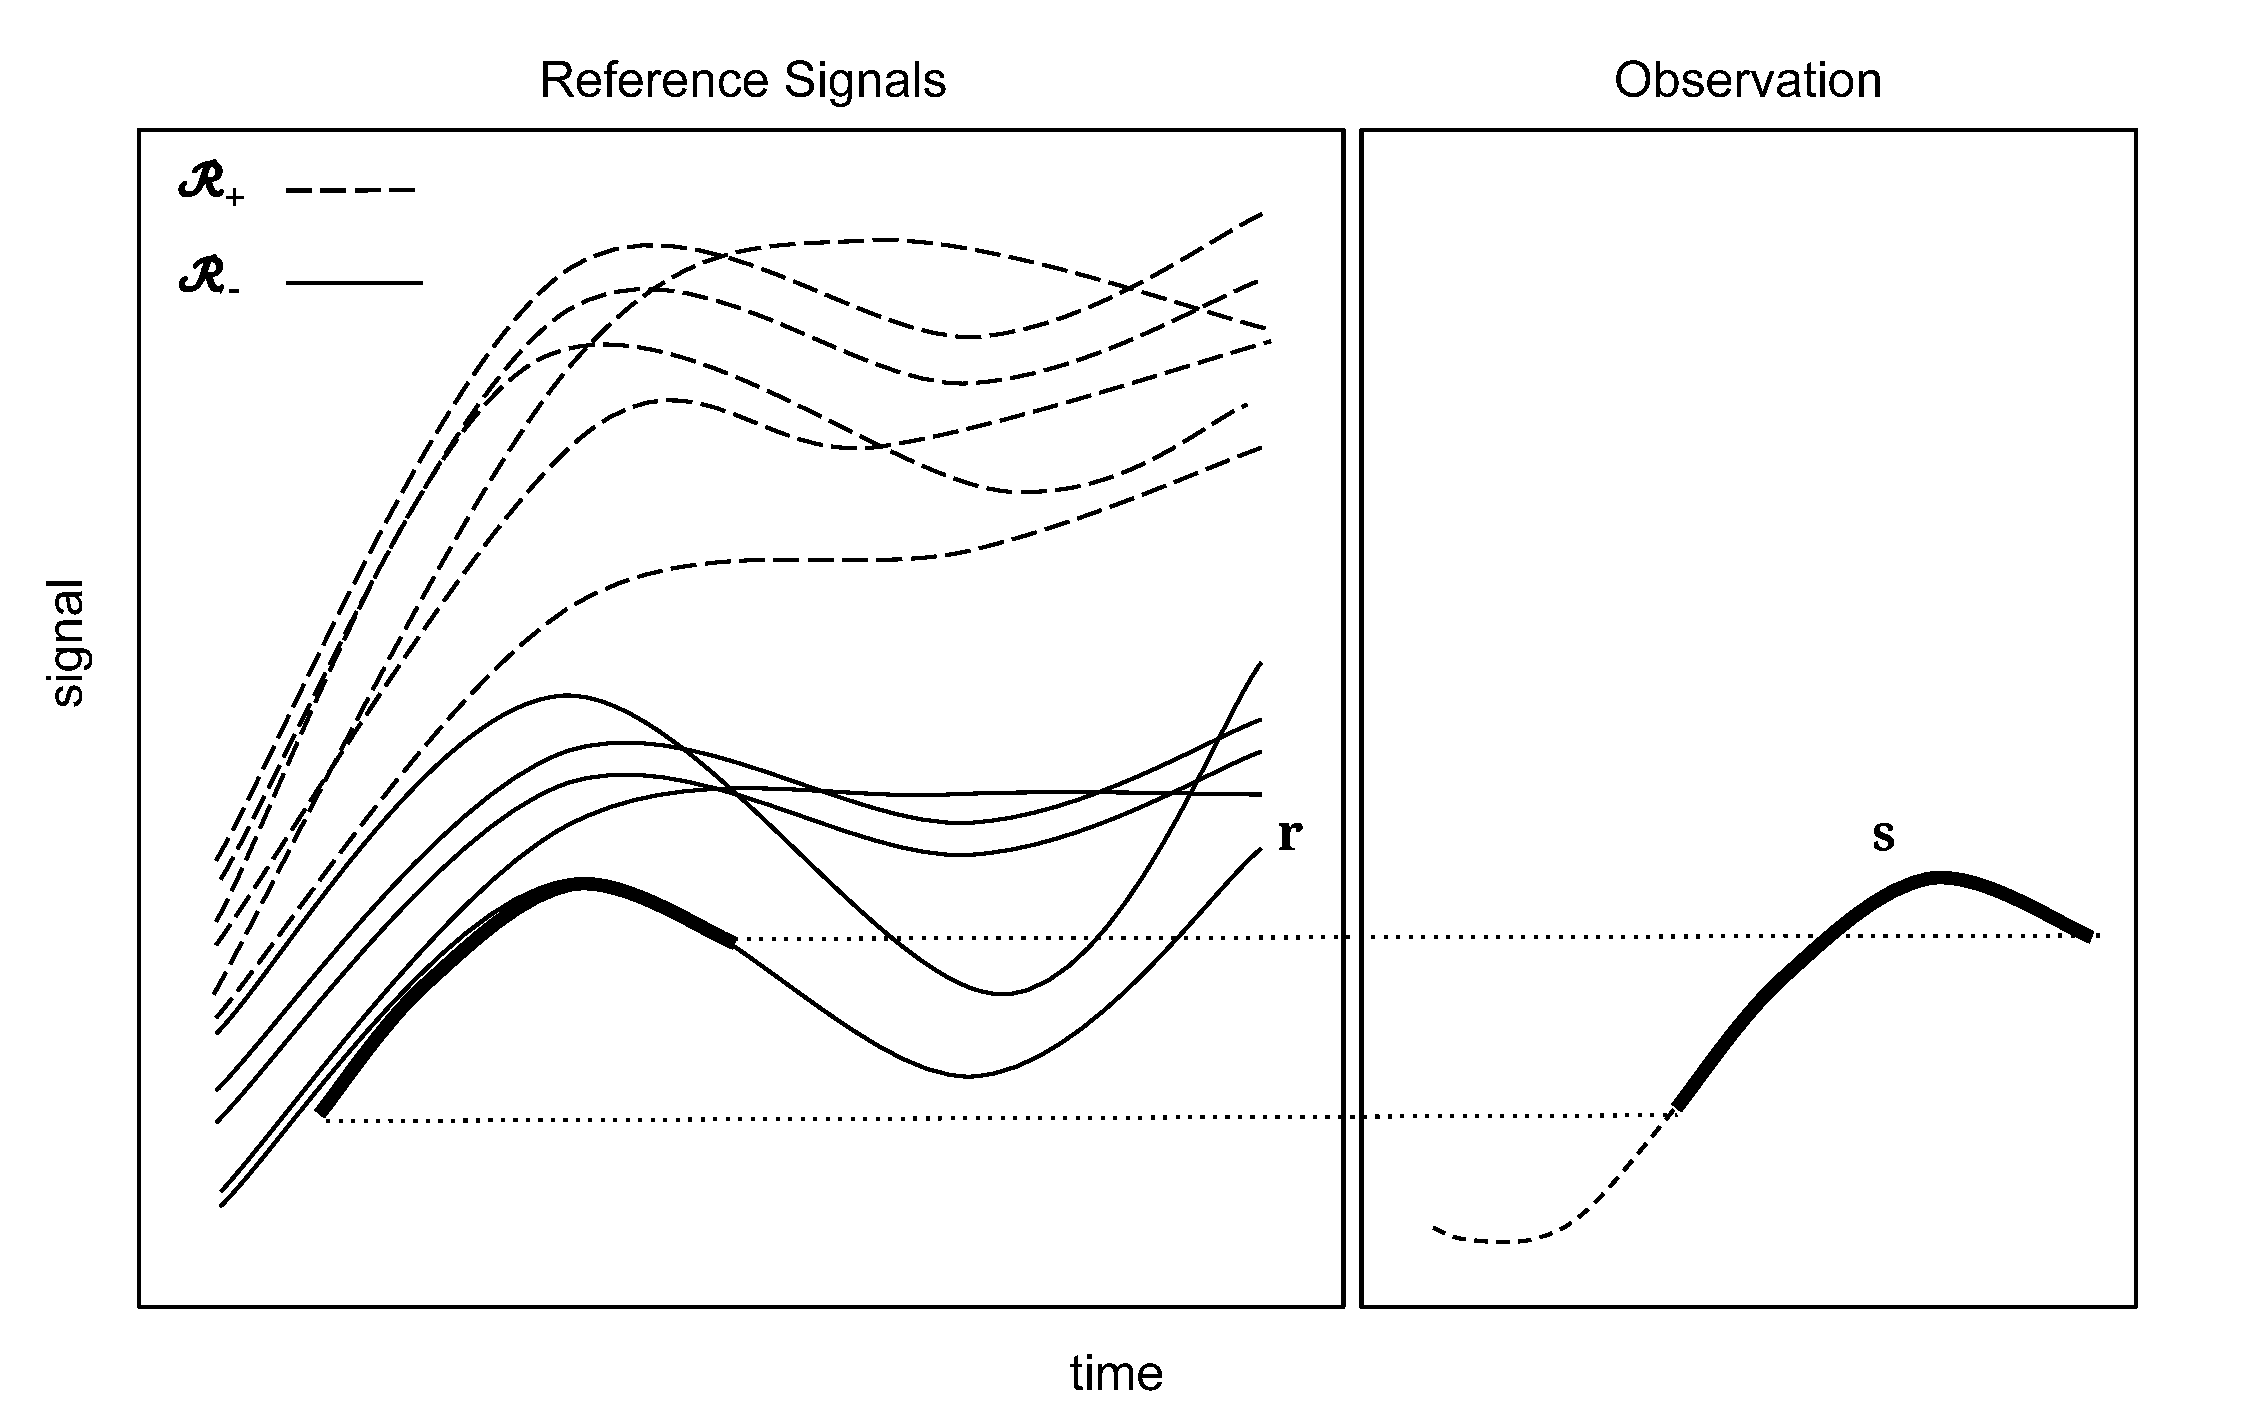
\includegraphics[width=6in]{mindist}
\end{center}
\caption{\label{fig:mindist} To compare a long reference signal to a short
  observation, we compute the distance between the observation (right) and the
  closest {\em piece} of a reference signal (left).}
\end{figure}

We generalize the distance function to reflect this
notion. Let us assume for simplicity that all observations are of length $N_{obs}$ and
all reference signals are of length $N_{ref} \geq N_{obs}$. We define the distance between a
reference signal $\mb r$ and an observation $\mb s$ as the minimum distance
between $\mb s$ and all contiguous subsignals of $\mb r$ of length $N_{obs}$.
\begin{gather}
d(\mb r, \mb s) = \min_{k = 1, \dots, N_{ref} - N_{obs} + 1} d(\mb r_{k:k+N_{obs}-1}, \mb s)
\end{gather}
Conveniently, for $N_{ref} = N_{obs}$, this new distance function reduces to the distance
function previously defined. Finally, using the generalized version of $d$, the ratio of
class probabilities $R(\mb s)$ from the previous section becomes
\begin{gather}
R(\mb s) = \frac{\displaystyle \sum_{\mb r \in \mathcal{R}_+} \exp \left(-\gamma \displaystyle \min_{k = 1, \dots, N_{ref} - N_{obs} + 1} \displaystyle \sum_{i=1}^{N_{obs}} (s_i - r_{i + k - 1})^2\right)}{\displaystyle \sum_{\mb r \in \mathcal{R}_-} \exp \left(-\gamma \displaystyle \min_{k=1,\dots,N_{ref}-N_{obs}+1} \displaystyle \sum_{i=1}^{N_{obs}} (s_i - r_{i + k - 1})^2\right)}.
\end{gather}

%TODO: 1-based indexing everywhere!!!

\subsection{A Remark on the Minimizing Latent Source}
It is possible to relax the assumption made in Eq. \ref{eqn:prob_plus_approx}
that the minimizing latent source $\mb t_{j^*}$ is close to the theoretically
best minimizer $\mb t^*$. A milder assumption would be that $\mb t_{j^*}$ is at
least {\em between} the reference signal $\mb r$ and the observation $\mb
s$. More precisely, let us assume that $\mb t_{j^*}$ is a point-wise convex
combination of $\mb r$ and $\mb s$:
\begin{gather}
\mb t_{j^*} = \mb A \mb r + (\mb I - \mb A) \mb s
\end{gather}
where $\mb A$ is a diagonal matrix with entries $\alpha_1, \dots, \alpha_{N_{obs}}$. If
$c(\mb x)$ can be further decomposed into
\begin{gather}
c(\mb x) = \sum_{i=1}^{N_{obs}} c_i(x_i)
\end{gather}
and scaling the argument of $c_i$ by a constant scales the output according to
\begin{gather}
c_i(ax) = g_i(a)c(x) 
\end{gather}
then $d(\mb s, \mb t_{j^*}) + d(\mb r, \mb t_{j^*})$ can be expressed as
\begin{align}
d(\mb s, \mb t_{j^*}) + d(\mb r, \mb t_{j^*}) &= d(\mb s, \mb A \mb r + (\mb I - \mb A)\mb s) + d(\mb r, \mb A \mb r + (\mb I - \mb A)\mb s)\notag\\
&= c(\mb A(\mb r -\mb s)) + c((\mb I - \mb A)(\mb r - \mb s))\notag\\
&= \sum_{i=1}^{N_{obs}} (g_i(\alpha_i) + g_i(1 - \alpha_i)) c_i(r_i - s_i).\label{eqn:weighted1}
\end{align}
Compare this to
\begin{gather}
d(\mb s,\mb r) = c(\mb r - \mb s) = \sum_{i=1}^{N_{obs}} c_i(r_i - s_i).\label{eqn:weighted2}
\end{gather}
Equations \ref{eqn:weighted1} and \ref{eqn:weighted2} show that $d(\mb t_{j^*},
\mb s) + d(\mb t_{j^*}, \mb r)$ is just a weighted version of $d(\mb r,\mb s)$
with weights $g_i(\alpha_i) + g_i(1 - \alpha_i)$ for $i = 1, \dots,
N_{obs}$. However, the weights depend on the particular $\mb A$ that defines the
convex combination. It is an interesting question whether $\mb A$ can be
inferred. However, this is outside the scope and purpose of this thesis.



%%%%%%%%%%%%%%%%%%%%%%%%%%%%% old
\begin{comment}
Suppose that $\Pi$ is the set of all possible events, $\Pi_+$ the set of all
possible viral events and $\Pi_-$ the set of all possible non-viral
events. Suppose that all events are disjoint, in the sense that no two events
can happen at once. Then if a viral event happens, it must be a noisy version of
exactly one of the events in $\Pi_+$.

We observe a signal and would like to determine if this signal was generated by
a topic that will become viral. To do this, we look at the signal for each
positive event and ask if the test signal was generated by the same type of
event that generated the positive event. We will assume that each signal was
generated by a seperate event in $\Pi$.
\end{comment}

